%$Id$
\documentclass[conference, compsoc]{IEEEtran}
\usepackage{fontspec}
%\usepackage{amsmath,amssymb,amsthm,supertabular,booktabs,rotating,semantic,subfigure,multirow,colortbl}
\usepackage{graphicx, url}
\usepackage[colorlinks=true,linkcolor=black,anchorcolor=black,citecolor=black,urlcolor=black,bookmarks=false,pdfstartview=FitH]{hyperref}
\usepackage{xunicode}
\usepackage{xltxtra}
\defaultfontfeatures{Mapping=tex-text}
\setmainfont{Times New Roman}
\begin{document}

\bibliographystyle{IEEEtran}

\title{Understanding software quality evolution using signifier frequency extraction}
\author{
Neil A. Ernst\\Dept. of Computer Science\\University of Toronto\\nernst@cs.toronto.edu \and
John Mylopoulos\\Dept. of Computer Science\\University of Toronto\\jm@cs.toronto.edu }

\maketitle

\begin{abstract}
We describe a repository mining technique we call signifier extraction. We generate signifiers using Wordnet and the ISO quality taxonomy. Using corpora created from eight Gnome projects -- their mailing lists, subversion comments, and bug comments -- we search for the signifiers over three month, quarterly intervals. The occurrence of our signifiers forms an evolutionary pattern that we analyze statistically and historically. We show that it is possible to reconstruct the historical evolution of project responses to external forcings, such as release cycles and audits. [numbers?]
\end{abstract}

\section{Introduction}\label{sect:introduction}
\begin{quote}[My impression] is of a large project in a state of marginal returns, in which a larger and larger part of the effort goes to maintenance. -- Andy Wingo, Gnome developer, June 2008.\footnote{http://wingolog.org/archives/2008/06/07/gnome-in-the-age-of-decadence}\end{quote}
	This quote, from a participant in the Gnome ecosystem (that is)
	
\begin{figure}[b]
\centering
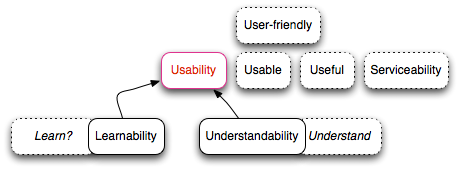
\includegraphics[width=0.4\textwidth]{synonym-graph.png}
\caption{An extensional definition of usability}
\label{fig:syngraph}
\end{figure}
	
	
\section{Signifier extraction}
In semiotics, Peirce first made the distinction drawn between signifier, signified, and sign~\cite{atkin2006}. In this work, we make use of signifiers -- words like `usability' and `usable' -- to capture the occurrence in our corpora of the signified -- in this example, the concept `usability'. We extract our signified, concept words from the ISO 9126 quality model~\cite{iso9126}. There is some debate about the significance and importance of the terms in this model. However, it is ``an international standard and thus provides an internationally accepted terminology for software quality~\cite[p. 58]{Boegh2008},'' which is sufficient for the purposes of this research. The model is used to refer to both external and internal views of quality (for example, bugs filed by users would be external qualities, whereas an email discussion of features to come would be internal). We generate the signifiers from Wordnet, a [] that contains semantic relations between words, including meronymy, synonymy, and holonymy. We extract words using the following criteria: [insert criteria]. This gives us a linguistic `bubble' which we use to extensionally define the signifier.

\section{Appendix}
Source code, data, and related discussions are available at \url{http://neilernst.net/msr09/}.
\begin{footnotesize}
\bibliography{msr}
\end{footnotesize}
\end{document}



